\question[4]
Ermittle mit dem Algorithmus von Dijkstra die kürzesten Wege von Knoten a zu allen anderen
Knoten.  Notiere die Reihenfolge der endgültig markierten Knoten.
Notiere für jeden Knoten die Reihenfolge der Werte, mit denen er markiert wird.

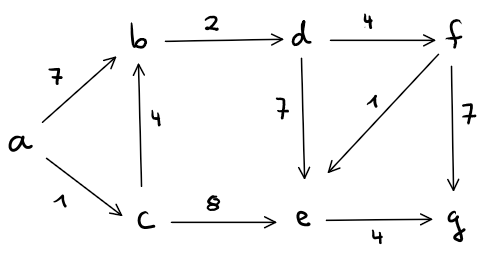
\includegraphics[height=4.3cm]{\pfad/Graphen/Aufgaben/dijkstra_06/dijkstra_06.png}
\begin{solutionbox}{5cm}
\begin{lstlisting}
Reihenfolge der endgültigen Markierungen: a c b d e f g
a : 0
b : inf 7 5
c : inf 1
d : inf 7
e : inf 9
f : inf 11
g : inf 13
\end{lstlisting}
\end{solutionbox}
